\chapter{Background} \label{ch:background}
\ifpdf
    \graphicspath{{Background/BackgroundFigs/PNG/}{Chapter3/BackgroundFigs/PDF/}{Background/BackgroundFigs/}}
\else
    \graphicspath{{Background/BackgroundFigs/EPS/}{Background/BackgroundFigs/}}
\fi

This chapter provides an extensive discussion over the problem of control in
packet-switched networks. We motivate the discussion over the problem of network 
control, describing firstly the architecture of existing network devices
(Section~\ref{sec:background:forwarding}) and  the currently-used mechanisms to
exercise network control in modern production networks
(Section~\ref{sec:background:netcontrol}). Motivated by the limitation of the
production solutions, we present three research network control schemes that
redefine the network control abstraction
(Section~\ref{sec:background:netcontrol}) and present
a number of proposed network control application that use these approaches and
and exercise evolved network control in specific network envi (Section~\ref{sec:background:ofapp}).

\section{Packet forwarding} \label{sec:background:forwarding}

Packet-switched networks have become a \emph{`de-facto`} technology in network
communication. Packet-switched network maximize medium utilization through their
inherent statistical multiplexing approach, while their simplicity significantly
reduces network costs.  In this section we focus on Ethernet and IP networks,
the predominant technology for packet switched networks, and we provide a
hardware design overview of two popular types of network devices: the {\it
  Switch } and the {\it Router}. 

\subsection{Switch}

\begin{figure}
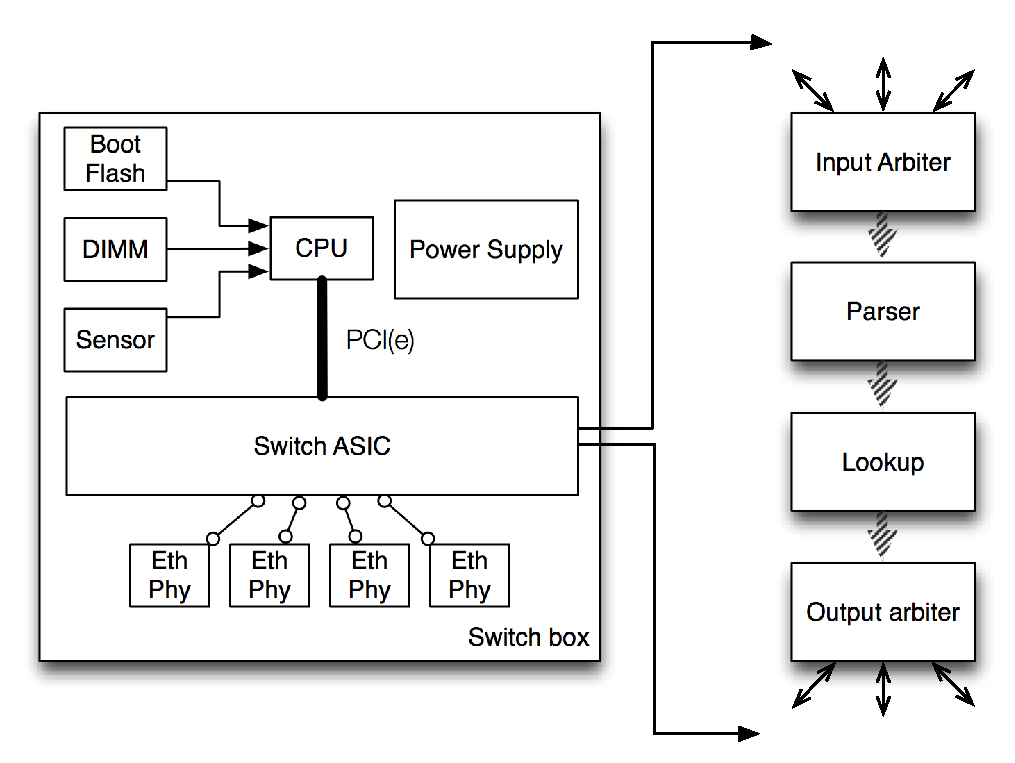
\includegraphics[width=0.9\textwidth]{switch_design}
\caption{A generic architecture of a Switching device.}
\label{fig:background:switch_design}
\end{figure}

Network switches are the main mechanism to multiplex Ethernet links.  This
device type provides collision-free connectivity between network segments and
use simple algorithms that minimize packet flooding.  Switches have multiple
functional roles in a network and as a result their architecture is highly
diverse. For
example, unmanaged switches provide a low cost non-configurable interconnection device 
for small networks, supporting usually multiple
1 gig ports, while core distribution switches are used in large enterprise
networks to interconnect aggregation switches, and support a few 10 or 40 Gig
links.  In this presentation we will use a simple switch type, the
Top-of-Rack~(TOR) switch.  This type of switch is used in datacenter network for
traffic agregation between the edges and the core of the network and provides,
at a minimum, learning-switch functionality. This switch type can forward
non-blocking high-rate traffic at line rate, using a single silicon chip. 
As presented in Figure~\ref{fig:background:switch_design}, a typical switch
device consists of the following components:

\begin{itemize}
  \item \emph{CPU}: Switch boxes contain a programmable CPU, which is used to
        run the control plane logic and provide reconfigurability to users.
        Switch vendors usually use low-power CPUs, such as SoC PowerPC chips or
        even ARM and MIPS CPUs. The CPU can access runtime memory
        module (Boot Flash and RAM), to store transient state, and persistent
        memory (e.g.~SD Cards) through memory extension slots, to store log
        files and configuration.
  \item \emph{Switch ASIC}: The Application-specific integrated
        circuit~(ASIC)~\cite{hp-asic,broadcom-asic,intel-asic} implements in
        hardware the forwarding plane of the switch.  The capabilities of an
        ASIC are variable, depending on the vendor and the cost, but define the
        functional limits of the device. In addition, fine implementation
        details of a ASIC silicon remain usually concealed, as they constitute an
        important asset for the silicon producer.  The development of a silicon
        design is a long process which takes years of development and testing,
        requiring extensive human and material resources. As a result, the
        introduction of novel functionality in the forwarding plane, is long and
        non-trivial and requires a significant amount of time. 

        TOR-type switches can handle
        line-rate non-blocking traffic for a few ports, using a
        single ASIC silicon.  Current ASIC contain four important modules.
        Firstly, the chip requires an {\it arbiter} module to multiplex and
        synchronize packet propagation from the Ethernet ports to the main
        processing pipeline of the silicon. The arbiter ensures non-preemptive
        packet processing, by bridging the rate mismatch between the 
        silicon clock and the transmission rate of the link. 
        In the main
        processing pipeline the ASIC requires a {\it protocol parsing} module and
        a {\it lookup module}. The protocol parser, extracts required packet
        fields, which are used later by the lookup module to define required
        packet processing.
        The lookup module relies on an interface with an external memory module
        in order to match protocol fields with policy packet processing.
        Memory modules have a trade-off between cost and access speed and a
        low-cost design principle can make the design extremely complex.
        \footnote{CAM/TCAM lookup: < 10 clock
          cycles, SRAM: 2-3 nsec, DRAM: 20-35
          nsec,~\url{http://people.ee.duke.edu/~sorin/prior-courses/ece152-spring2009/lectures/6.2.2-memory.pdf}}.
        Finally, the output arbiter is responsible to perform the required
        modifications to the packet and forward it to the appropriate output
        queue. Apart for the mentioned modules, a silicon can have additional
        processing modules to enable extended functionality such as access
        control list (ACL), flow statistics monitoring etc.
  \item \emph{ASIC-CPU communication}: CPU switching logic is integrated with
        the ASIC functionality over a PCI or PCI-express interconnection. Over
        this channel the firmware of the switch is able to control registers
        exposed by the ASIC, while the ASIC is able to inform the CPU of
        exceptional situations. The interconnection provides sufficient capacity
        to allow the CPU to poll the ASIC for statistics, or modify the
        forwarding process, but it sufficiently restricted to process forward
        plane traffic at high rates.
  \item \emph{Memory}: Apart for the in-ASIC memory modules, modern switches
        also use multiple memory types in order to provide a computational
        environment similar to a PC. An average switch will contain Boot Flash,
        to boot the OS/firmware, DIMM RAM, to accommodate the run-time main
        memory of the firmware, and multiple memory slots, to provide low
        capacity storage to the firmware in order to persist switch logging and
        configuration.
  \item \emph{Ethernet ports} : The receipt and transmission of Ethernet packets
        is implemented as a separate hardware module. The module is responsible
        to implement the physical layer protocol. In addition the modules may
        also contain packet buffers to reduce packet losses for bursty traffic.  
    
\end{itemize}

In this case we present a simple switch case that can support average traffic
requirements on the edges of the network. Higherer-end Switches, establish more 
complex hardware design, in order to modularize further
functionality and enable multi-port Terrabyte traffic. An extensive discussion
over hardware architecture of Cisco switches is presented in~\cite{cisco-routers}.

\subsection{Router}

A router device is used to interconnect Ethernet networks, at the IP level.
Router device follow similar hardware design, as in the case of Switches. 


\section{Forwarding Control} \label{sec:backoground:netcontrol}

Network control is an important aspect of network functionality, as it enables
dynamic adaptation of network devices.  A number of protocols and mechanisms have 
been introduced to provide resilient and distributed network control. In this section
we will present standardized, as well as, research protocols and architectures
that aim to provide dynamic network control.

\subsection{Routing and switching}

Current network control plane technologies have been influenced extensively by the
end-to-end principle of the Internet. A switch or a router control logic
requires only its local state, and a number of distributed protocols
enable state exchange between devices, in order to construct a better view 
of the network and increase forwarding policy efficiency. The
device persists only its local state between reboots and the available protocols
allow dynamic recreation of the global state, thus achieving long-term
network resilience.  In this section we present existing production-level protocols that
enable distributed network control. We focus on Ethernet and IP networks, as
these are the predominant network protocol and we follow the natural split in
Data-Link layer and Network layer protocols, as these two layers have fundamentally
distinct characteristics.

\subsubsection{Switching control protocols}

Data-Link layer control protocols aim to provide loop-detection, and VLAN and
QoS automation. Loop detection is used to avoid packet loops in networks with
redundant connectivity, since Ethernet packet format doesn't provide packet
timeout functionality. IEEE standardised the STP protocol in the IEEE
802.1D-1998~\cite{ieee_802_1d}; a distributed Spanning Tree calculation
mechanism, based on the algorithm defined in~\cite{Perlman1985}. The algorithm
uses broadcast messages to discover a spanning tree over the graph of the
network, with respect to a root switch. The protocol defines a state machine per
port, which can disable packet forwarding if a port is detected to cause loop.
Because the initial definition of the protocol incurred high latency in Spanning
Tree calculation after a network change, IEEE introduce RSTP, an evolve version
of STP, in~\cite{ieee_802_1d_2004}.  The STP mechanism was also evolved to
address the requirements of VLAN configuration. VLAN tagging can create multiple
different subgraph over the network and individual STP runs over each subgraph
can increase network utilization. This functionality is provided by IEEE
Multiple Spanning Tree Protocol (MSTP)~\cite{ieee_802_1q}, while Cisco has
developed a series of proprietary protocols~\cite{pvst,pvst+}.  Finally, IEEE
has recently defined an advanced STP protocol that enables switches to discover
and use in parallel redundant network links, in the IEEE 802.1aq
standard~\cite{ieee_802_1aq}.

In terms of automatic configuration, network vendors and standardization bodies
have developed a number of protocols that can disseminate information to
neighbouring nodes and ease device management. Such protocols have high
churn between vendors and each vendor defines its custom standard. In this
class of protocols we consider Link Layer Discovery Protocol (LLDP), supported
by IEEE, Cisco Discovery Protocol (CDP),  Extreme Discovery Protocol, Nortel
Discovery Protocol. Finally,in order to reduce the administation
burden of VLAN trunk links between switch, Cisco has developed the VLAN Trunking Protocol
(VTP).

In the class of Data Link layer protocols we also consider the MPLS
protocol~\cite{RFC3031}. The MPLS technology tries to bridge the gap between
virtual-circuit technologies, like ATM, and packet-switched networks. MPLS
reduces the ATM control plane complexity and removes the limiting small capsule
size. MPLS forwarding relies on tunnel labels which simplifies the lookup
functionality in the silicon and reduces memory requirements. MPLS is used
extensively in the distribution layer of large networks. In order to automate
the configuration of MPLS circuits, the protocol use the LDP
protocol~\cite{RFC5036}, which sets up labels across the network. In order to
enable resource control over MPLS tunnels, IETF has defined a mechanism to map
RSVP resource control over the MPLS label management~\cite{RFC3209}.  Because
MPLS doesn't provide a mechanism to control resource allocation, resource
control is implemented using a mechanism called {\it Autobandwidth}.
Autobandwidth monitors tunnel bandwidth requirements and recalculates paths when
bandwidth requirements change. A study on a deployment of this technology in the
MSN network though has highlighted that the allocation policy is commonly
short-term under-optimal~\cite{Pathak2011}.

% In Data-Link layer we can also consider the MPLS protocol 

\subsubsection{Routing control protocols}

In the network layer, modern network technologies exercise control through
routing protocols. Routing protocols follow a similar approach to Data Link
layer protocols and provide mechanisms to disseminate local configuration to the
network. Basic routing protocols are split in {\it Link State}, {\it Distance
  Vector} and {\it Path Vector} protocols. Link state protocols build on-top of
the Djikstra algorithm~\cite{Djikstra1959}. Routers disseminate local
forwarding configuration to all participating routers in order to construct the
global graph and using each router calculate the minimum
spanning tree of the network, using Djikstra's algorithm.  IETF has defined the
OSPF protocol~\cite{2328}, an Ipv4 specific routing protocol, while the
Open Systems Interconnection~(OSI)
organisation has defined the IS-IS protocol~\cite{RFC1142}, a network technology
agnostic routing protocol.
Link state routing protocols provide the framework to develop highly flexible
routing mechanisms as each router has view over the complete graph of the
network. Link State protocols can disseminate multiple
link metrics to other routers, but the decision mechanism must be
homogenus across the network for loops and packet loss avoidance.

Distance Vector routing protocols use a different routing approach. Routing
information is exchanged only between adjacent routers, and the global optimal
paths are slowly propagated across the network. This type of routing algorithm
relies on the Belman-Ford algorithm~\cite{bellman1956}. The RIP
protocol~\cite{RFC2453} has been developed to provide Distance Vector routing in
networks, while Cisco has developed the proprietary IGMP
protocol~\cite{Rutgers1991}. Distance Vector protocols are less extensible than
Link State routing protocols, but can be implemented with smaller computational and
memory requirements.

Path Vector routing protocol try to address some limitation of the Distance
Vector protocols for Interdomain routing. In Path Vector routing, adjacent
routers advertise for a specific destination the list of ASes that a packet will
traverse towards that subnet, instead of a signle weight. As a result, Path
Vector routing protocols can encapsulate the routing policy of an AS and expose
only paths for a destination. Using this information, administrator can define
routing policies and configure their edge routers. The BGP
protocol~\cite{RFC1265} implements Path Vector routing.

Distributed network control provide modern network excellent resilience during
unexpected network changes. The routing algorithm have been mathematically
proved to find optimal solution, when a solution exists. Nonetheless, the
control abstraction of these protocol is not a good fit to exercise
dynamic control by the administrators. In 2008 the global Internet was severely
affected by a BGP misconfiguration from the Pakistani national
ISP in an effort to control traffic from YouTube service~\cite{bgp_config_error}. 
In addition, the latency of the protocols
to respond to network events can impact significantly network performance.
For OSPF, authors in~\cite{Watson2003} monitor OSPF
functionality in a regional ISP and report high churn in routing even during
periods without significant network events, while the latency to converge after
a network change is common to be on the order of seconds. Similar results have
been observer in BGP. In~\cite{Kushman2007} the authors highlight a strong 
correlation of BGP instability and VoIP performance. 

\subsection{Active Networks}

The problem of protocol ossification in the network layer and the requirement
for network evolvability, started to become interesting for the network research
community
in mid 90's. In~\cite{O'Malley1992}, the authors argue on the generality of the
7-layer OSI network abstraction. They claimed that the networks functionality
should be more dynamic and forwarding devices should be able to accommodate
variable number of protocol layers. In their work they present an extensible protocol
modeling framework to layer protocol processing. Motivated by these observations, DARPA
funded the {\it Active Networks} project~\cite{darpa_active_net}, in an effort
to develop next generation extensible network devices. 

Active networks modify the traditional mechanism of packet processing and
introduce the notion of {\it capsules}. Capsules are network packets that carry both data
as well as processing code. On each hop, the default packet
processing logic is extended with the code contained in the packet, thus
redefining network functionality. This network processing approach provided
user-driven protocols upgrades, without upgrades of 
inter-mediate network devices.  In addition, the development of novel
programming languages, like Java, provided sufficient uilding blocks to implement such
approaches.  

Research in active networks tried to define two mechanisms : the {\it capsule
  API and format} and the {\it switch architecture}. In terms of capsule
format, the active network community defined the Active Network Encapsulation
Protocol~(ANEP)~\cite{alexander1997a}.  ANEP, due to its format specification,
made a clear separation between functionality and data. An Active Node using a
new protocol would inject firstly new processing logic, using code capsules, and then
send the data stream, as data capsules.  The format was adopted by the ANTS and
Sprocket frameworks.  Sprocket~\cite{Schwartz200} was an effort to develop an
efficient capsule programming language by BBN technologies. The language uses a
restricted set of the C language, avoiding any security vulnerable structures
like pointers, while it introduced native support of SNMP browsing. Sprocket
compiled source code to compact MIPS assembly. Each switch would receive code
capsules and run the code in a MIPS virtual machine. The VM could not persist
any state on the switch, but it was able to modify the data section of a packet.
Finally, security was implemented using a public key secure hash of the code,
but without sufficient details on the authentication logic.
ANTS~\cite{Wetherall1998} was the attempt of MIT to develop an equivalent
framework. ANTS used a restricted version of the Java language to program
capsules, mainly due to the ability of Java to serialize object state, while
the processing logic was modeled through a small number of Java interfaces. ANTS
permitted injected code to store reduced information in the switch, as
well as, modify state of packets. An interesting extension of the ANTS framework
was the code dissemination mechanism. An
end-node deployed new protocol functionality solely to the local Internet
gateway, and the code is forwarded along with the packets to each
next-hop. Finally, The university of Pensylvania active networks group developed
its own approach to capsule programming.  PLAN~\cite{Hicks1998} used a restricted
version of the OCaml language which allowed packets to access the local switch
resources and implement custom forwarding logic. PLAN did not follow the ANEP
packet format. A PLAN capsule contains
code and data, while the code section would replace the network header
information. In order to secure switch infrastructure, the language
disallowed  packet data modification or switch state persistence. The language 
aimed to provide a framework to define the control plane of the device.

In terms of Active Network platforms architecture, the community developed a
number of architectures, addressing multiple aspects of efficient protocol
processing. University of Pensylvania proposed the SwitchWare Execution
Environment (EE)~\cite{Alexander1998}.  The architecture defined an OCaml module
framework for capsule processing. A core focus of the SwitchWare EE was strong
multi-dimension security for active networks, both on the local system, as well as, on
the capsule execution.  SwitchWare used SANE~\cite{Alexander1998b}, a
trustworthy operating system, to secure the functionality of the switch, and
build on top of it multiple security guarantees. The platform addressed issues
regarding secure execution and authentication, while also providing primitives
to verify capsule code.
PLANet~\cite{Hicks1999} and Active Bridge~\cite{Alexander1997b} used the
SwitchWare framework and implemented novel functionality over an active network. 

The active networks group in University of Arizona proposed its custom approach
for efficient efficient active network platforms. Their approach relies on the Scout
OS~\cite{Montz1995}, a communication-oriented OS supporting efficient
layered data processing. On top of Scout, the group developed the Liquid Software
API~\cite{Hartman1999}. The integration of Liquid Software API and Scout, aimed to
establish a tight integration between the OS and the JVM and improve capsule
processing, using the JIT JAVA compiler. 

The CANEs project~\cite{Chae2002} from Georgia Tech Active Networks groups
followed a different approach for the problem and designed a system which
enabled multi-protocol packet processing. CANEs defined a number of
abstractions, which enabled active network applications to stack multiple
protocol processors on the forwarding path. CANEs project build on top of the
Bowman Switch OS~\cite{merugu1999} and established a simple and efficient
abstraction over the Switch resources. 

Researchers from the Columbia University, presented the NetScript switch
abstraction~\cite{daSilva2001}. NetScript is a new programming language
optimized for flexible protocol processing definition and composition. The
project defined three types of protocol composition: layered composition,
composition through protocol bridging and end-to-end composition. This approach 
permitted developers to extend flexible extension of protocol processing. 

Finally, a joint effort between the Network Laboratory of ETH and the University
of St. Louis, proposed the development of the High Performance Active Network
Node (ANN) switch architecture~\cite{Decasper1999}. The project aimed to develop a high performance
active network system and proposes the introduction of an FPGA for each ATM
interface and offload protocol processing to the FPGA. Using this
infrastructure, the researchers where able to run the ANTS EE and develop an
IPv4 and IPv6 protocol processor to run in Gigabit rates. 

Active network research put forward a number of interesting insights on the
controllability and evolvability problem of computer networks functionality.
Nontheless, the introduced complexity and extreme clean-slate design made it
difficult for the approach to reach the production environment. Active Network
functionality was highly benefited from the relatively low rate of the network
rates of the time, but the rapid evolution in network rates made it impossible
to sustain efficient implementations that could cope with multi-Gigabit rates. 

\subsection{Tempest Switchlets}

\begin{figure}
  \begin{center}
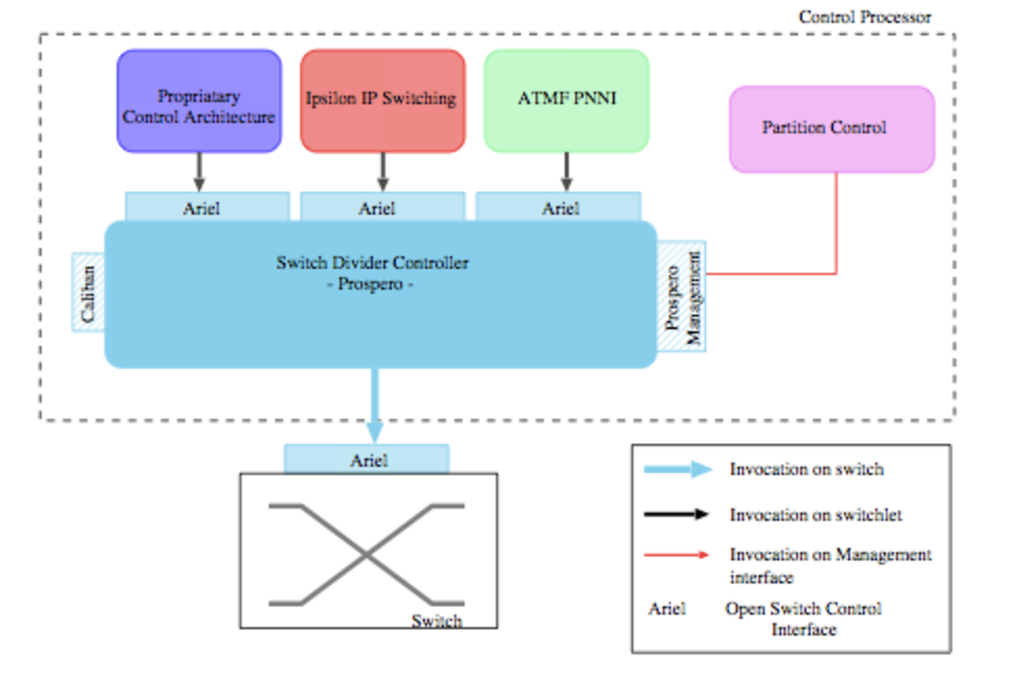
\includegraphics[width=0.7\textwidth]{tempest_arch}
\caption{Tempest switch architecture~\cite{UCAM-CL-TR-450}}
\label{fig:background:tempest_arch}
\end{center}
\end{figure}

An effort for network programmability in ATM network was also developed in the
University of Cambridge, as part of the DCAN~(Devolved Control ATM Networks)
project~\cite{dcan}.  The system, called Tempest~\cite{Rooney1998}, aimed to
provide dynamic control of network resource virtualization. Tempest provides a
clear separation between the control and forwarding plane of a network device.
The control plane is outsourced in other devices, in order to aggregate control
from multiple switches and implement intelligent and dynamic forwarding over a
virtual network of switches.  A similar approach is followed by the OpenFlow
protocol over Ethernet networks.  The implementation of Tempest is logically
divided between three abstractions, depicted in
Figure~\ref{fig:background:tempest_arch}. The Figure presents how a single
switch is able to function in parallel as an IP router, an ATM switch and 
Hollowman controlller~\cite{Rooney1997}, a devolved ATM control framework. 

\paragraph{Prospero Switch Divider} 

The {\it Prospero} abstraction provides a mechanism to virtualise ATM switch
resources. Prospero exposes a service able to partition switch resources and
create multiple virtual switches, called {\it switchlets}. A switchlet controls
a subset of the switch ports and VCI and VPI mappings. In terms of buffer and
bandwidth virtualization, Prospero reuses the inherent ATM QoS principles. This
layer is also responsible to map the interface exposed to the controllers with
the underlying switch functionality. 

\paragraph{Ariel Switch Independent Control Interface} 

Network control entities can control the switchlet forwardind using the Ariel
Interface. The interface defines the functionality that a switchlet should
provide to a controller along with a protocol specification. Ariel defines five
control objects: {\it Configuration}, {\it Port}, {\it Context}, {\it
  Connections} {\it Statistics} and {\it Alarms}.  Configuration provides
details for the current configuration of the switch, Port provides primitive
controllability of ports (e.g.~state, loopback functionality), Context permit
isthe controller to define QoS policies, Connections expose VPI/VCI mappings,
Statistics exposes packet and byte counters and Alarms push state change
notifications to the controller. Any Tempest switch runs an Ariel server and
translates Ariel request to the Prospero layer. 

\paragraph{Caliban Switch Management Interface}

Apart from control capability support, Tempst also defines mechanisms for
network management over the switchlet abstraction. The management is defined
through the Caliban interface. The interface is similar to the functionality of
the SNMP protocol, but also defines, apart for the fine level information that
SNMP provide, higher level aggregation information. 

In addition to the redefinition of the network control abstraction, Tempest also
promoted the adoption of a relaxed network resource management scheme.
Specifically, the architecture proposed a measurement-based admission control
for new circuit~\cite{Lewis1998}. The measure scheme relied on effective
bandwidth measurement techniques. This approach allowed better utilisation of
available resources. 

Tempest defined a very elegant framework for network control and modern
SDN approaches have adopted a large number of functionalities. The framework
avoided the idea of code execution on forwarding devices, thus addressing
significant security concerns of the active network approach, and defined a
simple forwarding plane, which was able to run at line rate in existing
hardware. Nonetheless, its strong reliance to the ATM technology makes it a bad
fit for modern Ethernet-dominant network technologies. 

\subsection{SDN}

Software Defined Defined (SDN)~\cite{sdn} networking is a novel approach for scalable 
and flexible network control. Software defined networking focuses on a single
observation that there is a clear split between the control and the data plane
of a network device. Data Plane refers to the packet forwarding functionality of the system
, while Control Plane refers to the logic behind this forwarding logic. 
\subsubsection{OpenFlow protocol}

\section{Control Plane Applications} \label{sec:background:ofapp}
\subsection{Datacenter network}
\subsection{Home network}
\subsection{Wireless network}
\subsection{Simulation}

\section{Conclusions}
